\documentclass[dvipsnames]{article}
\usepackage[margin=0.8in,letterpaper]{geometry}
\usepackage{graphicx}
\usepackage{amsmath,amssymb}
\usepackage{authblk}
\usepackage[T1]{fontenc}
\usepackage{gentium}
\usepackage{newtxmath}
\usepackage{natbib}
\usepackage[final]{hyperref}
\usepackage{tikz}
\usepackage{xcolor}
\usepackage{fancyhdr}
\usepackage{siunitx}
\usepackage{titlesec}
\usepackage{multicol}

\setcounter{secnumdepth}{4}

% A schematic for data processing might be helpful
\usetikzlibrary{shapes,arrows}
\tikzset{font=\footnotesize}

\newcommand{\sg}[1]{{\color{MidnightBlue}{{[SG: \bf #1]}}}}
\newcommand{\dl}[1]{{\color{Plum}{{[DL: \bf #1]}}}}
\newcommand{\gs}[1]{{\color{WildStrawberry}{{[GS: \bf #1]}}}}
\newcommand{\yz}[1]{{\color{OliveGreen}{{[YZ: \bf #1]}}}}

\pagestyle{fancy}
\fancyhf{}
\rhead{East Coast Regional Virtual Datathon Fall 2020}
\lhead{S. B. Green, D. Li, G. Schumacher, and Y. Zhang}
\cfoot{\thepage}

\hypersetup{
	colorlinks=true,       % false: boxed links; true: colored links
	linkcolor=Orchid,        % color of internal links
	citecolor=Orchid,        % color of links to bibliography
	filecolor=Orchid,     % color of file links
	urlcolor=Orchid         
}

\renewcommand\Affilfont{\itshape\small}

\title{%

\includegraphics[width=0.5\textwidth]{data-open-logo.jpg}~
\\[1cm]
East Coast Regional Virtual Datathon Fall 2020 \\[0.1cm]
\large Team 19} 
\author[1]{Sheridan B. Green}
\author[1]{Daming Li}
\author[1]{Grant L. Schumacher}
\author[2]{Youyuan Zhang}
\affil[1]{Department of Physics, Yale University}
\affil[2]{Department of Mathematics, Courant Institute, New York University}


\date{September 20, 2020}

\graphicspath{{figures/}}

\begin{document}

\maketitle

\section{Topic question}
An accurate understanding of consumer movie preferences is crucial for effectively guiding production, marketing, investment, and, ultimately, the prosperity of the film industry. In this report, we leverage several datasets, which include movie metadata, consumer ratings, and Academy Award nominations, in order to explore the following questions:
%
\begin{enumerate}
    \item Are there any genre-dependent temporal evolution patterns and statistical features present in consumer movie ratings?
    \item How predictive are user rating statistics with respect to Academy Award nominations, and, conversely, how do such nominations end up reshaping future user rating statistics?
\end{enumerate}
%
The answers to these questions could help guide film production companies to develop successful movies that target specific consumer groups and are released at the optimal times based on prevailing macroscopic genre preferences. These questions are especially relevant given the shift away from traditional media and towards online platforms.  With these questions and goals in mind, we combine predictive modeling and causal inference techniques to extract insight from existing consumer preference information and provide recommendations regarding the positioning of future movies for film makers and investors.

\section{Executive summary}

Guided by the questions above, our analysis of the data yields several significant insights.

We begin with an exploratory analysis of various rating statistics and temporal patterns of movie rating evolution from the year 1995 through 2018, breaking down the data by genre (we discuss the results of Figs.~\ref{fig:eda1} and \ref{fig:eda2} in the current and subsequent paragraphs). We find that some genres have consistently higher mean ratings (such as crime and drama) whereas some genres have consistently lower ratings (such as comedy and science fiction). This suggests that some types of films are more likely to be ``crowd-pleasers'', reflecting different levels of production difficulty across genres. In addition, the temporal evolution of the mean ratings across years is highly non-stationary but largely synchronized across genres. The seasonality of monthly rating data, however, is weak.

The non-stationarity of the mean ratings is an interesting phenomenon, as it might be driven by exogenous macroscopic variables. These may be unexpected social or natural events resulting in an impulsive change, or more slowly varying economic factors related to welfare and technology infrastructures. The fact that the chronological correlations between genres are high may be due to the fact that many movies belong to multiple genres. We also find that there is, on average, a decreasing trend in the rating as a function of years after the release of a movie. Such a trend is particularly significant for comedies, whereas it is not present at all for genres such as drama and thriller. We interpret this as the fact that some types of content are closely associated with the context and epoch in which they are created, and such a link becomes weakened as time passes by. This again shows that certain genres of movie are intrinsically harder to make than others, and that certain genres have a much shorter ``shelf life''. We use the fraction of total ratings associated with movies of each genre per year as a proxy for the evolving genre ``market share''. We find that dramas have consistently attracted the most reviews over time, but that action and fantasy movies have been steadily gaining market share since the early 2000s. Until recently, comedies were the second most reviewed (now overtaken by action), but their prevalence has been dropping dramatically over the past 15 years.

Besides the above descriptive analysis, our modeling work provides insights into the bi-directional interactions between consumer ratings and Oscar nominations. 

First, we build a classification model incorporating features such as rating count, mean rating, and standard deviation of ratings of a given movie immediately after its release to predict its probability of being nominated for an Academy Award (results summarized in Table~\ref{tab:logistic}). Consistent with intuition, the rating count is shown to be positively associated with this probability: popular movies with more reviews tend to be more successful. The mean rating also has a positive regression coefficient: high quality movies have a better chance for awards. We highlight the role of the rating standard deviation by asking the following: given two movies with the same average rating, is the one with a larger standard deviation more likely to be nominated? We find that this feature has a significant negative slope of dependence. This suggests that movies should target a broader audience to increase their chances of being nominated.

Next, we investigate whether the chance of nomination depends on film genre by adding binary genre features into the existing predictive model described above. We find that the prediction accuracy is significantly improved after taking genres into consideration. Some movie genres tend to have a higher probability of being nominated, such as dramas, while some genres of movies tend to have a lower chance, such as thrillers. Consequently, movie makers aiming at winning Oscar awards should carefully choose the genre and content of the production.

The predictive model we have built illustrates how a film's genre and early reviews can predict Oscar nominations. But there is also another direction of association: do Oscar nominations induce any changes in average ratings of movies? We calculated the mean causal effect using ratings immediately before and immediately after the nomination announcements, comparing the change in mean ratings between Oscar nominated-movies and those that were not (see Fig.~\ref{fig:mc}). We find that on average there is a weak, yet significant drop in mean rating after a movie is nominated (mean causal effect size of -0.04 with $p=5\times 10^{-5}$). This drop is consistently present in nearly all genres of movies (but is strongest in comedy, drama, and romance). This is interesting, and the actual reason is worth further exploration. A possible reason might be that after a movie is nominated, it raises peoples' expectations for the movie before watching it, while at the same time the audience is more easily upset about the quality. On the other hand, we did not observe any significant change in the variance of ratings after Oscar nominations.

Based on our results, we make the following recommendations for movie makers and investors. Some movie genres (such as comedies) seem intrinsically harder to successfully produce compared to others. Furthermore, the favorability of individual genres has a considerable magnitude of time evolution. Therefore, if the stakeholders primarily care about reputation and financial success, it would be wise to carefully consider genre when considering a new production. Additionally, if a movie maker aims to be nominated for or even win an Academy Award, they may want to engage a broader audience rather than making a film that specifically targets a subset of consumers.

\section{Technical exposition}

\subsection{Data and preprocessing}

In this work, we use several publicly available datasets provided to us that, when taken together, enable a robust analysis of the film industry over the past several decades. The \href{https://grouplens.org/datasets/movielens/}{MovieLens database} \citep{MovieLens} contains ${\sim}$27 million ratings and ${\sim}$1.1 million tag applications that cover ${\sim}$58 thousand movies and come from ${\sim}$280 thousand distinct users of the \href{https://movielens.org/}{MovieLens site} collected over the year range of 1995 to 2018. While the crowd-sourced MovieLens data does indeed provide a \textit{lens} into the public perception of various films, there is perhaps a more authoritative indication of a movie's success, which comes in the form of a nomination and potential conferral of an Academy Award (i.e., an Oscar). Thus, we also use a \href{https://www.kaggle.com/unanimad/the-oscar-award}{dataset} that contains information about every Oscar nomination and award from 1927 through 2018. 

These datasets contain a massive amount of data and are not in the exact form needed for our modeling purposes initially. Hence, in what follows, we describe the necessary preprocessing steps that we perform prior to analysis.

The titles of the movies in the \texttt{movies.csv} MovieLens file do not exactly match those in the \texttt{the\_oscar\_awards.csv} file. For example, in the former file, the article, ``The'', is always placed at the end of the title; the title itself is followed by the release year of the film, which is concatenated onto the same string. Thus, we wrote a function to clean the film titles in order to match the convention of the other files. Furthermore, each movie can belong to multiple genres, which are initially pipe-separated in the \texttt{genres} column. We separate the genres of each movie entry by converting the string to a list, which is then associated with the corresponding movie as a column in a \texttt{pandas} DataFrame.

The \texttt{ratings.csv} file contains the ratings that users have submitted for movies that they have reviewed; each rating has a corresponding timestamp. We extract the year and month from each timestamp for the purpose of time series analysis. Next, the ratings table is merged with the movies table. Not all movie genres receive an equal number of ratings (see Fig.~\ref{fig:eda2}). When investigating genre-dependent properties, we only include the nine genres with at least 300,000 total ratings, which we least in decreasing order by rating count: Drama, Comedy, Action, Thriller, Adventure, Romance, Sci-Fi, Crime, and Fantasy. The time courses of mean rating evolution by genres were obtained by calculating the ratings averaged across users and movies in each month.

The \texttt{the\_oscar\_award.csv} contains a list of all movies that have been nominated for an Oscar between 1927 and 2018. Since the MovieLens data only contains information beginning in 1995, we limit ourselves to Oscar-nominated movies from 1995 onward in our analysis.

Other model-related feature engineering and/or transformations are explained in the corresponding modeling subsections below.


\subsection{Exploratory data analysis}

In order to gain some initial understanding of the film data at hand, we begin our analysis by calculating some descriptive summaries of the MovieLens user review data. Each review entry consists of a user ID, movie ID, five-star rating, and timestamp. We group the reviews by user ID, which enables us to compute the mean and standard deviation of ratings on a user-by-user basis. We then repeat this process, instead binning by movie ID, which yields a mean and standard deviation of ratings for each movie. In Fig.~\ref{fig:eda1}, we show the distribution of review counts as well as mean and standard deviation of reviews per user and per movie. Interestingly, the distribution of review counts by user peaks at ${\sim}70$ and has a tail that extends out to the low thousands --- we suspect that the reviews from this minority of users with such high rating counts could potentially be used to represent the opinions of a ``movie critic'' user group. The distribution of review counts for movies is heavily right-skewed, with the maximum reaching roughly 100,000 reviews. The mean user rating is roughly at 3.6, whereas the mean movie rating is lower at 3.1. In general, movie ratings tend to have a standard deviation of roughly 1.0 about their user/movie mean.

\begin{figure}
    \centering
    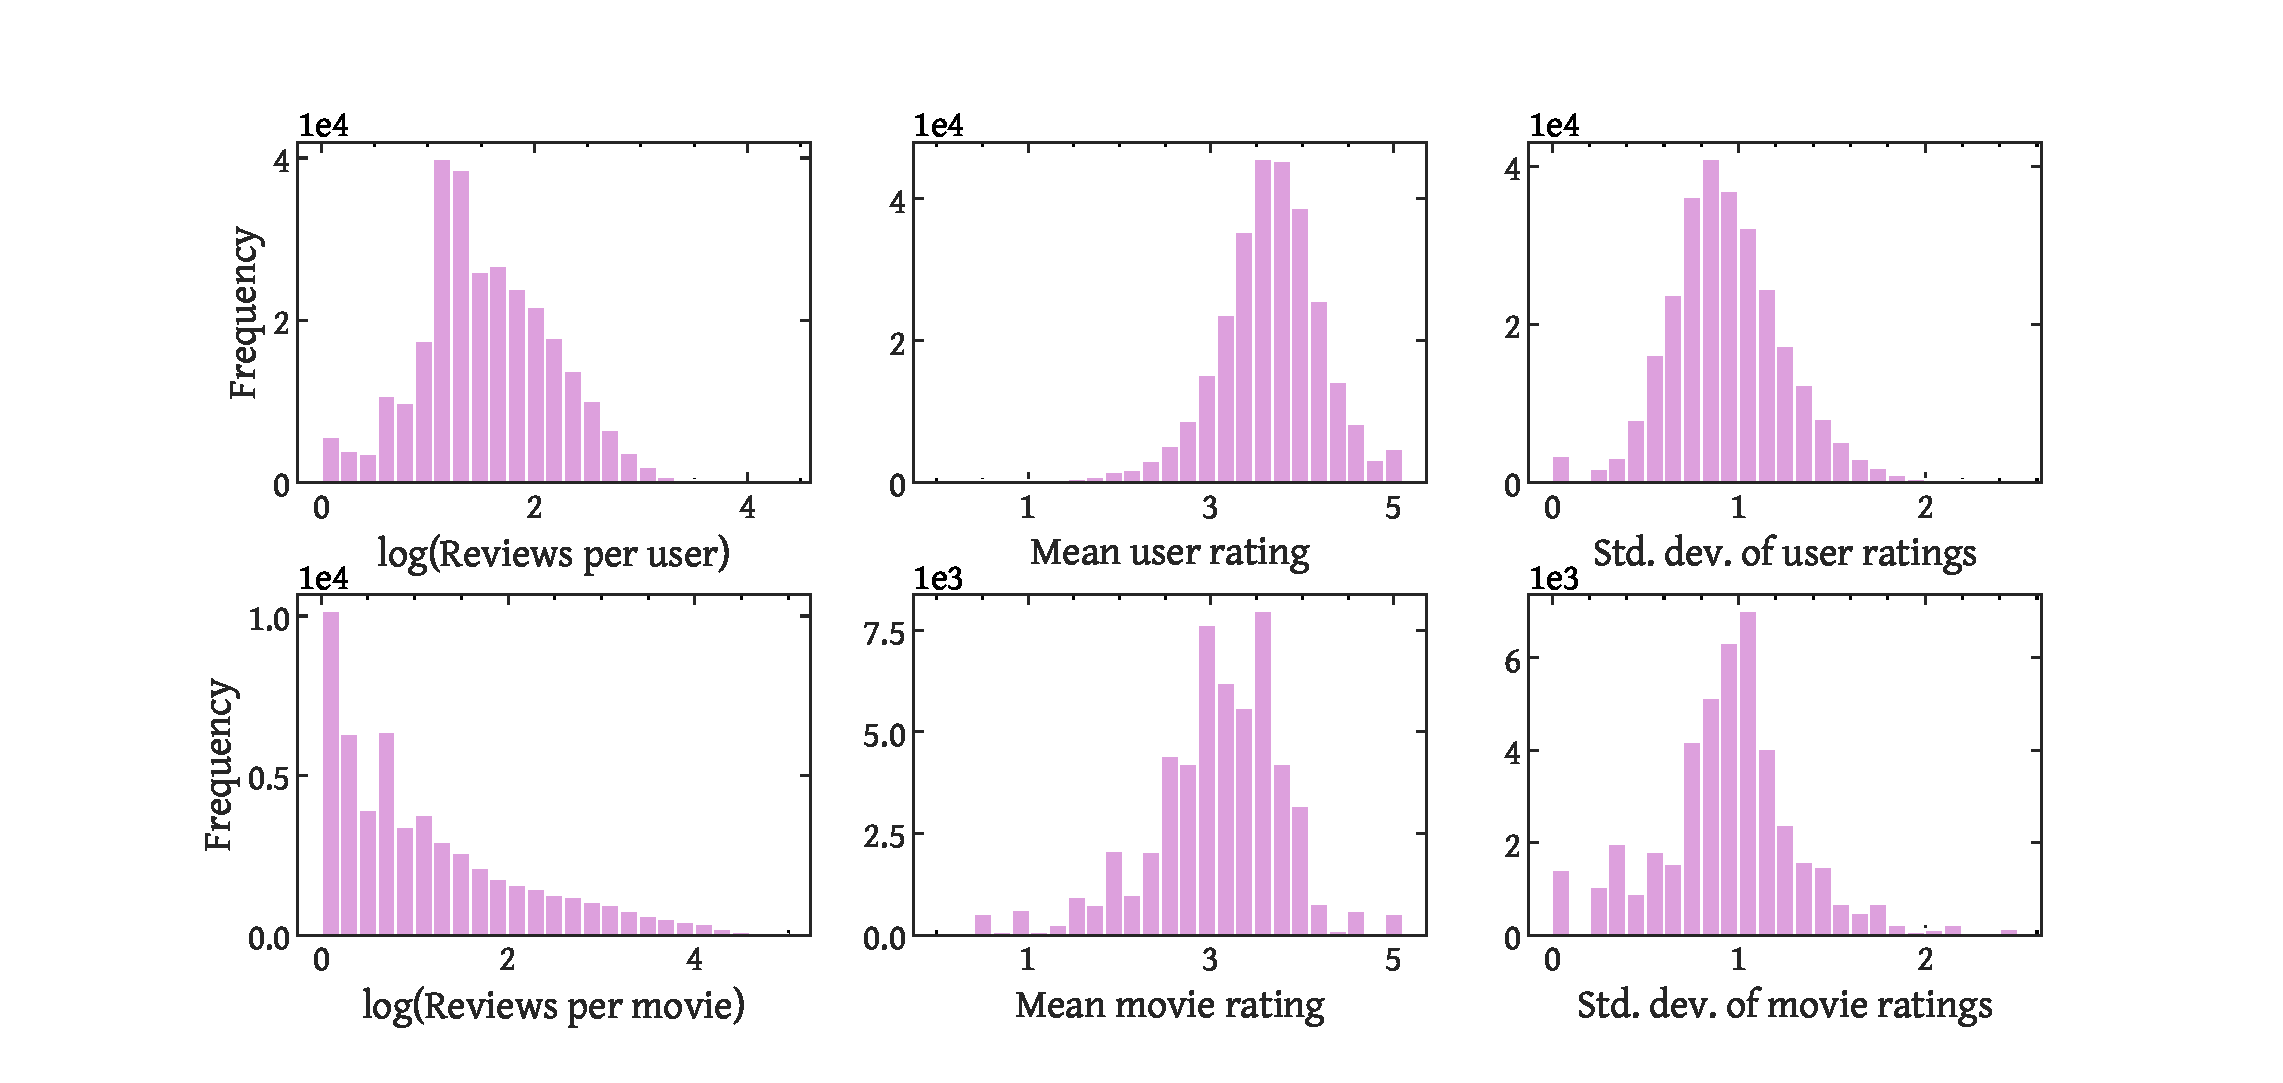
\includegraphics[width=\textwidth]{movielens_eda1.eps}
    \caption{Descriptive rating statistics aggregated by user ({\it top row}) and by movie ({\it bottom row}).}
    \label{fig:eda1}
\end{figure}

As a next step in our exploration, we direct our attention to the temporal trends seen in the MovieLens ratings. At this point, we begin to perform analysis on a genre-by-genre basis. In Fig.~\ref{fig:eda2}, we show several salient genre-dependent temporal trends observed in the ratings. In the upper right panel, we show the evolution of the yearly mean in movie ratings from 1998 to 2018 broken down by genre. This is computed by grouping all user ratings by year and then secondarily by genre and taking the mean within each group. Most noticeably, the temporal trend in the mean ratings is highly synchronized across genres, while modulated by exogenous factors. However, it is clear that drama and crime films are consistently the highest rated, whereas comedies are consistently the lowest rated. In order to look further into the synchronization between genres, we instead compute the monthly mean per genre and then measure the pair-wise Pearson correlation between the rating time series of each genre (spanning 1997 to 2018). We illustrate this as a correlation matrix heatmap in the upper left panel. The genres are arranged into groups based on their correlations --- comedy, drama, and romance fall into a tightly correlated group whereas the remaining genres fall into a separate, fairly highly correlated group. The correlations are overall very high because a movie can belong to multiple genres. In the middle panel, we look more deeply at the monthly fluctuations by grouping all user ratings by movie. The box plots show the distribution of user-averaged ratings per movie as a function of month (for the year of 2017) and grouped by genre. Here, we see the genre-dependent standard deviation in movie ratings and note a fair level of consistency in ratings from month to month, albeit with mild fluctuations. Overall, we find that monthly seasonality of ratings over the years is minimal. Interestingly, this seems to contradict the film industry's assumed wisdom, namely that blockbuster action films are better received when released in the summer.

\begin{figure}
    \centering
    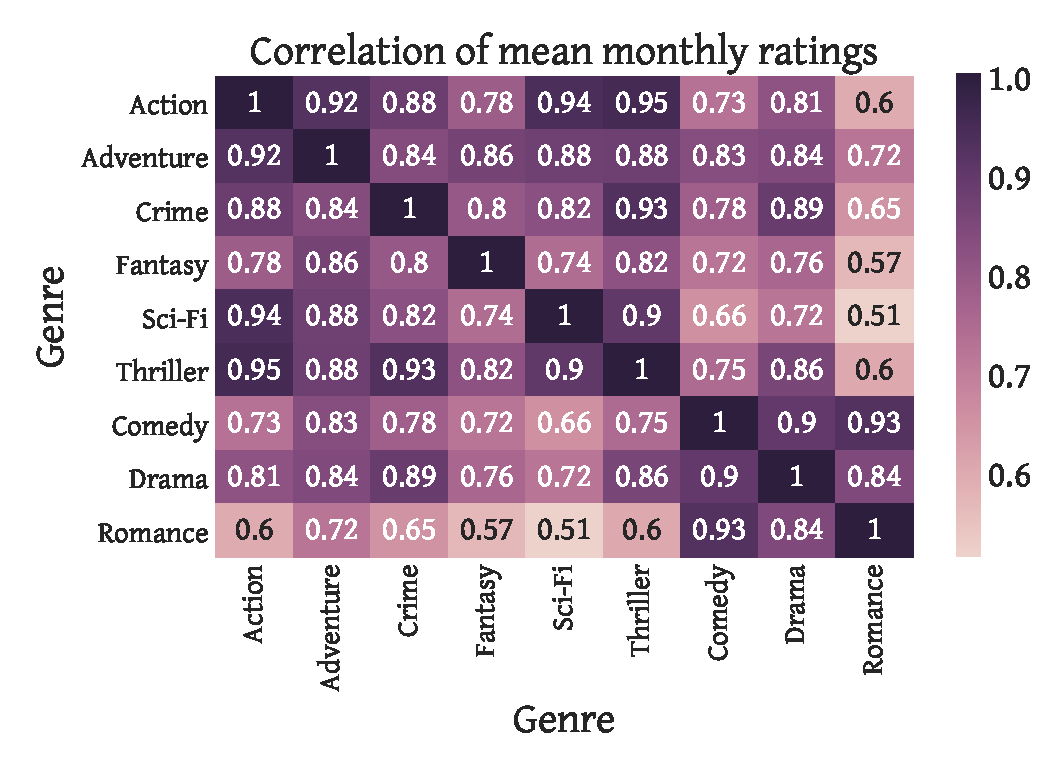
\includegraphics[width=0.47\textwidth]{hm.eps}
    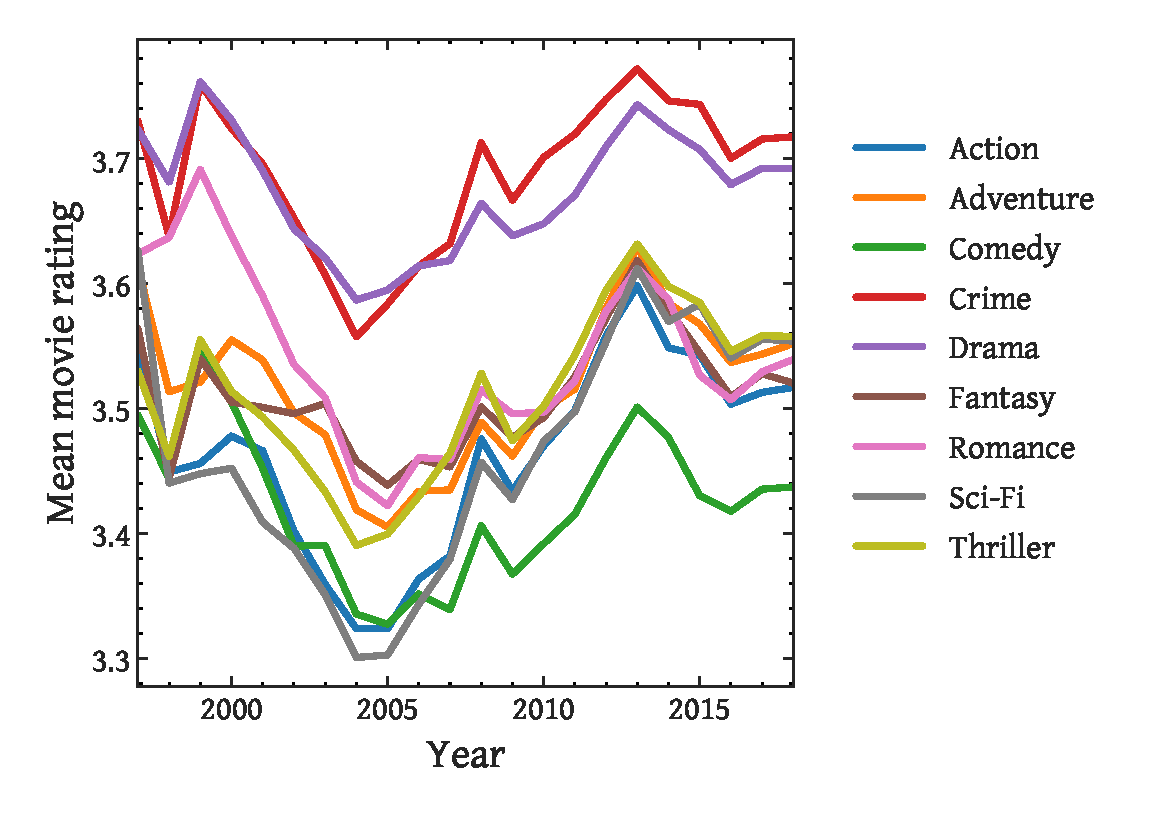
\includegraphics[width=0.47\textwidth]{ty.eps}\\
    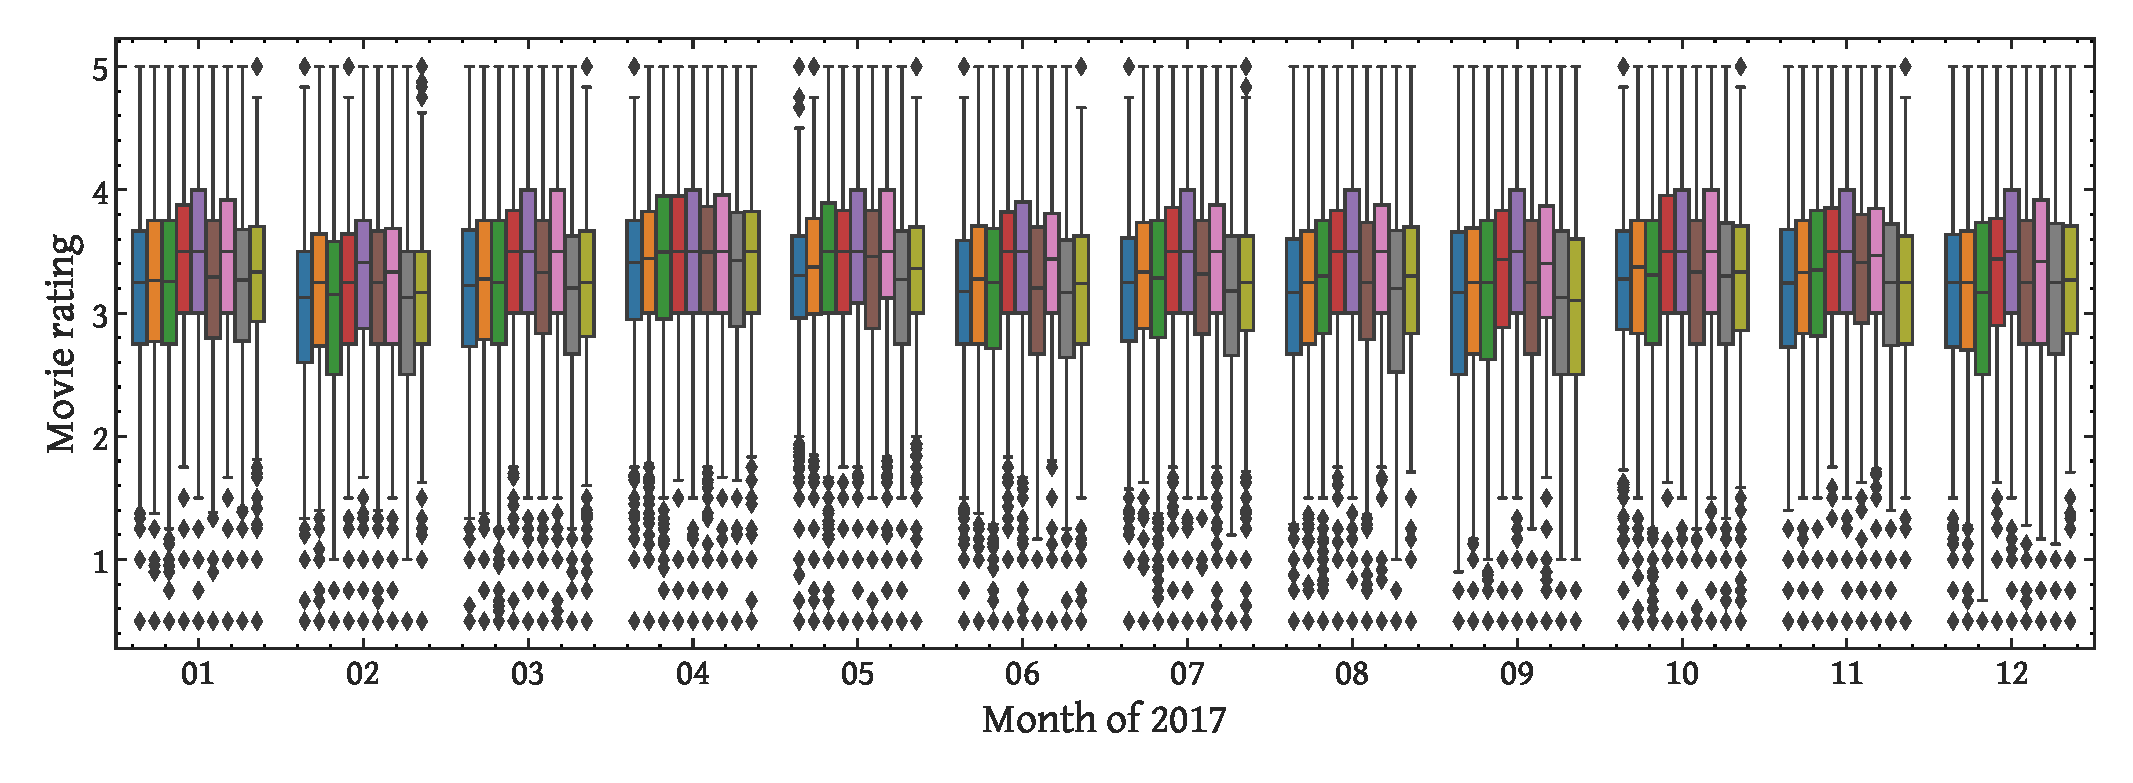
\includegraphics[width=\textwidth]{mp.eps}\\
    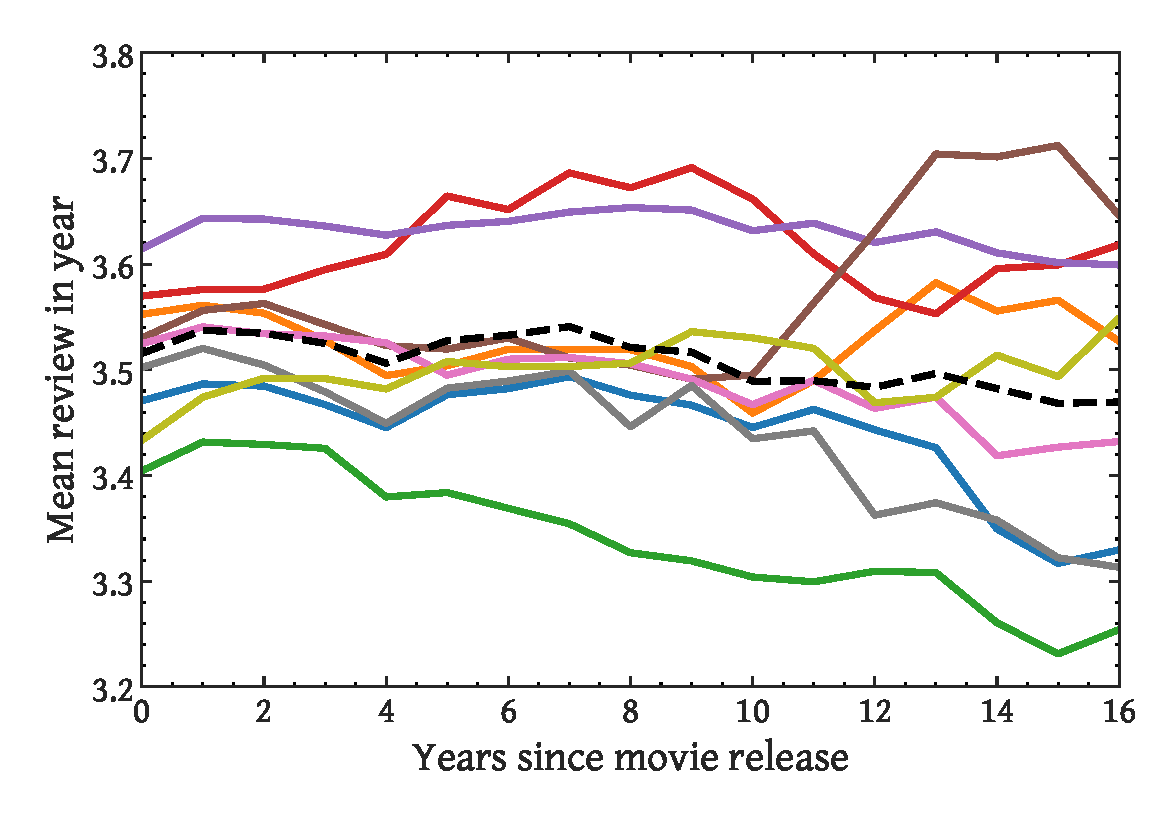
\includegraphics[width=0.47\textwidth]{mvy.eps}
    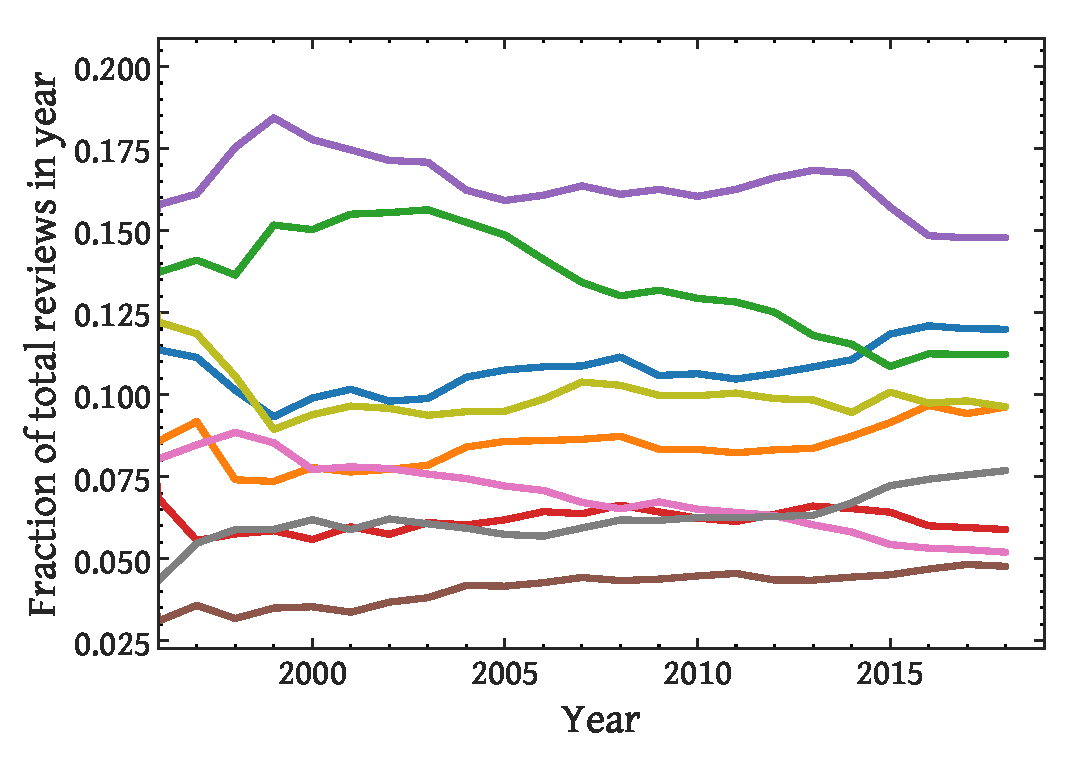
\includegraphics[width=0.47\textwidth]{fpy.eps}
    \caption{Rating evolution separated by genre. {\it Top Left:} A heatmap that illustrates the (monthly) temporal correlation between the mean MovieLens ratings of different genres (spanning from 1997 through 2018). {\it Top Right:} Mean rating from year 1998 through 2018. Note that the color scheme used for the different genres is consistent across all panels. {\it Middle:} Monthly movie ratings throughout the year of 2017, where each data point represents a movie's mean rating averaged over its reviewers. {\it Bottom Left:} Mean rating evolution as a function of years since a movie's release. The dashed black curve corresponds to the mean aggregated over movies across all genres. {\it Bottom Right:} Temporal evolution of the fraction of total reviews associated with films of each genre.}
    \label{fig:eda2}
\end{figure}

In order to understand how well the public opinion of films withstands the test of time, we perform the following analysis. We restrict ourselves to movies that premiered from 2000 onward, since the MovieLens yearly rating count after 1999 is considerably higher than in the earliest years of ratings data. For each movie with release date of 2000 or more recent, we use the timestamp of its first rating as an approximation of the specific date of release. Then, we compute the time since movie release for each rating by taking the time difference between the rating and the first rating of the corresponding movie. We bin all reviews by the number of years since movie release and measure the mean rating in each bin. In the lower left panel of Fig.~\ref{fig:eda2}, we show the evolution of the mean movie review as a function of years since release (black dashed line); we also further break this trend down by genre. The trend indicates a small, but non-negligible, decrease in mean movie ratings as a particular film ages. We note that this is a well-known phenomenon, which has even been discussed in an \href{https://help.imdb.com/article/imdb/track-movies-tv/why-do-the-user-ratings-on-many-movies-and-tv-shows-seem-to-decrease-over-time/G4SK7DG5EA35B4GF}{article on IMDb}. When separated by genre, the temporal decline in ratings is much more significant and is strongest for comedy, action, and sci-fi films. We suspect that the action and sci-fi film ratings likely hold up poorly over time due to the constant improvement of special effects in films. On the other hand, the dramatic decline in mean comedy ratings over time since release could be attributed to various forms of humor falling out of favor in the public eye that depended on, for example, offensive or culturally insensitive content that was more prevalent in older films. In order to confirm whether there is, in fact, a meaningful trend in the reviews as a function of time since film release, we run an augmented Dickey-Fuller test for stationary (with cutoff $p=0.05$) on the time series results. These tests show that the overall mean trend is \textit{not} stationary. When broken down by genre, only action, crime, and thriller films pass the test for stationarity.

When planning a movie production, an important metric to consider is the overall popularity of the proposed genre at the time of release. Such a quantity is important to consider when estimating the size of the target consumer audience. The ``market share'' of a particular genre can be estimated by the fraction of total reviews given that are associated with films of that genre. Hence, in the lower right panel of Fig.~\ref{fig:eda2}, we show the time evolution of this review fraction, binned by year. Notably, dramas have consistently held the largest market share since the inception of MovieLens. Historically, comedies also have held a dominant market share, but it has declined significantly over the past ${\sim}15$ years. Action movie dominance appears to be on the rise, which is most likely spurred by the proliferation of superhero movies in recent years. Similarly, fantasy films have shown a slow but consistent increase in market share over the past two decades. An important note is that this approach does not consider the values of the actual ratings, but simply their abundance --- one could even argue that the ``success'' of a film depends more on its ability to garner viewers than on its actual evaluation by those viewers.

Motivated by the MovieLens descriptive summaries and the rich genre- and time-dependent structure seen in our exploration of the ratings data, we identify several directions to extend our analysis. Since the mean of, variance in, and count of ratings varies widely from film to film, we would like to see if these quantities are predictive of movie ``success''. There are various metrics for success, but a simple, binary metric is whether or not a movie is nominated for an Oscar. Since Fig.~\ref{fig:eda2} demonstrates that the market share and mean rating varies widely across genres, we are also interested in exploring the extent to which a movie's genre is predictive of its ability to be nominated for an Oscar. Our finding that mean ratings decrease over time raises an additional question: can being nominated for an Oscar help combat this gradual decay in a movie's ratings, does it have no effect, or does it exacerbate the decline? We explore these questions in the following subsection.

\subsection{Modeling}

\subsubsection{Predictive modeling of Oscar nominations}

\paragraph{Role of rating statistics}\label{ssssec:lr}

We aim to build a predictive model that can provide insight into how consumer ratings for a particular movie influence the probability of it ultimately being nominated for an Oscar. Since receiving a nomination is itself a significant accolade, we will refrain from modeling whether or not the Oscar was actually awarded. For each movie, we consider three factors in our model: (i) the total number of user ratings, (ii) the mean rating, and (iii) the standard deviation of the ratings. The rating count is a proxy for the movie's popularity and its attention received by consumers. The mean rating reflects the overall degree to which the audience enjoyed the movie. Lastly, the standard deviation of the ratings captures the variation in opinions towards the movie among different consumer groups. We included this last covariate because we are interested in addressing the following question: given that movie A and movie B have equal mean ratings whereas movie A received more varied ratings among users, is movie A more or less likely to be nominated for an Oscar than movie B? 

The Academy Awards typically consider movies that were released in either the same year or the year before the awards ceremony. For this reason, user ratings must be chosen carefully based on their timestamps. First, we limit our analysis to movies released after the year of 1998, since the overall abundance of MovieLens reviews is much larger from 1999 onward. For Oscar-nominated movies, we only include ratings that were recorded in the year prior to the ceremony; if there were no ratings during the previous year, we instead use ratings made during the same year as the ceremony. The purpose of this step is to minimize target leakage caused by including data after nomination announcements. Similarly, for movies that were not nominated, we only include ratings within one year after their release.

The prediction of nomination probability is an imbalanced classification task. In our dataset, 845 out of 14,133 (i.e., the sample size) movies were nominated. Therefore, we adopt a logistic regression model with a resampling technique in order to address this issue. Specifically, we call the total number of ratings $\mathbf{rating}\_\mathbf{cnt}$, the mean rating $\mathbf{rating}\_\mathbf{mean}$, and the rating standard deviation $\mathbf{rating}\_\mathbf{std}$. Then, the nomination of an Oscar is modeled as a Bernoulli event with a probability of $p$, whose logit (i.e., log-odds) is modeled as
%
\begin{equation}
    \ln \frac{p}{1-p} = \beta_0 + \beta_1 \times \log_{10}(\mathbf{rating}\_\mathbf{cnt}) + \beta_2 \times \mathbf{rating}\_\mathbf{mean} + \beta_3 \times \mathbf{rating}\_\mathbf{std} .
\end{equation}
%
Here, the $\beta_i$ are our regression coefficients. We use the logarithm of $\mathbf{rating}\_\mathbf{cnt}$ because the distribution of rating counts is heavily right-skewed and spans several orders of magnitude. We use the standard deviation of the ratings rather than variance in order to have consistent ``units'' (i.e., ratings rather than ratings$^2$) between $\mathbf{rating}\_\mathbf{mean}$ and $\mathbf{rating}\_\mathbf{std}$.

We first split the sample into a training set and a test set with a size ratio of $3:1$. Next, we up-sample the minority class (i.e., nominated movies) in the training set such that the resulting abundances of nominated and non-nominated movies are balanced. We fit a logistic regression model to this balanced training data and subsequently use the model to predict nominations in the test set. We obtain the regression coefficients, $p$-values, and an ANOVA table using existing procedures available in R (\texttt{glm} and \texttt{anova.glm}). The prediction accuracy is assessed using the recall (the ratio of correctly identified true positives to the sum of true positives and false negatives) and area under the receiver operating characteristic curve (ROC AUC) scores. 

The left hand side of Table~\ref{tab:logistic} summarizes our fitting results. All three covariates are significantly associated with nominations. The ANOVA table demonstrates that adding the three covariates sequentially does indeed significantly improve the fit. The nomination probability logit is positively associated with rating count and rating mean, whereas it is negatively associated with the rating standard deviation. As for prediction accuracy when applied to the test data, our model attains a recall of 0.705 and an ROC AUC score of 0.7.

\begin{table}
    \centering
    \setlength\columnsep{5pt}
    \begin{multicols}{2}
    \begin{tabular}{|c|S[table-format=-1.3]|S[table-format=-1.3]|c|}
    \hline
    {Covariate} & {Coefficient} & {Std. Err.} & {$p$-value} \\
    \hline
    Intercept      & -5.897 & 0.167 & $<2\times 10^{-16}$  \\
    $\log_{10}(\mathbf{rating}\_\mathbf{cnt})$ &  1.341 & 0.022 & $<2\times 10^{-16}$  \\
    $\mathbf{rating}\_\mathbf{mean}$          &  1.168 & 0.041 & $<2\times 10^{-16}$  \\
    $\mathbf{rating}\_\mathbf{std}$       & -0.591 & 0.069 & $<2\times 10^{-16}$  \\
    \hline
    \end{tabular}
    \vspace{4em}
    
    \begin{tabular}{|c|S[table-format=4.1]|c|}
    \hline
    {ANOVA} & {Deviance} & {$p$-value}  \\
    \hline
    $\log_{10}(\mathbf{rating}\_\mathbf{cnt})$ & 7987.7 & $<2\times 10^{-16}$ \\
    $\mathbf{rating}\_\mathbf{mean}$          & 1440.3 & $<2\times 10^{-16}$ \\
    $\mathbf{rating}\_\mathbf{std}$       &   74.1 & $<2\times 10^{-16}$ \\
    \hline
    \end{tabular}
    %
    \begin{tabular}{|c|S[table-format=-1.3]|S[table-format=-1.3]|c|}
    \hline
    {Covariate}  & {Coefficient} & {Std. Err.} & {$p$-value} \\
    \hline
    Intercept    &  -5.220  & 0.172 & $<2\times 10^{-16}$  \\
    $\log_{10}(\mathbf{rating}\_\mathbf{cnt})$ &   0.635  & 0.011 & $<2\times 10^{-16}$ \\
    $\mathbf{rating}\_\mathbf{mean}$    &   0.972  & 0.042 & $<2\times 10^{-16}$        \\
    $\mathbf{rating}\_\mathbf{std}$     &  -0.674  & 0.070 & $<2\times 10^{-16}$        \\
    $\mathbf{is}\_\mathbf{Action}$    &  -0.578  & 0.066 & $<2\times 10^{-16}$          \\
    $\mathbf{is}\_\mathbf{Adventure}$ &   0.621  & 0.070 & $<2\times 10^{-16}$          \\
    $\mathbf{is}\_\mathbf{Comedy}$    &  -1.069  & 0.048 & $<2\times 10^{-16}$          \\
    $\mathbf{is}\_\mathbf{Crime}$     &  -0.071  & 0.067 &     0.293                    \\
    $\mathbf{is}\_\mathbf{Drama}$     &   0.422  & 0.040 & $<2\times 10^{-16}$          \\
    $\mathbf{is}\_\mathbf{Fantasy}$   &   0.077  & 0.083 &     0.354                    \\
    $\mathbf{is}\_\mathbf{Romance}$   &  -0.004  & 0.055 &     0.943                    \\
    $\mathbf{is}\_\mathbf{Sci\_Fi}$    &  -0.599  & 0.085 &  $2.3\times 10^{-11}$       \\
    $\mathbf{is}\_\mathbf{Thriller}$  &  -1.015  & 0.058 & $<2\times 10^{-16}$          \\
    \hline
    \end{tabular}
    \end{multicols}
    \caption{A summary of the logistic regression results. {\it Left top}: Regression coefficients and their significance for the model with only rating-related covariates. {\it Left bottom}: ANOVA table for the rating-only model, which is created in an add-on manner. {\it Right}: Regression coefficients and their significance for the genre-dependent model.} 
    \label{tab:logistic}
\end{table}

\paragraph{Dependence on movie genre}

The predictive model introduced in Section~\ref{ssssec:lr} only includes statistics of user ratings as covariates. However, we are also interested in whether the results are genre-dependent. For example, movies of which genre are most likely to be nominated? In order to investigate this, we follow the same procedure as above, replacing the regression function by
%
\begin{equation}
    \ln \frac{p}{1-p} = \beta_0 + \beta_1 \times \log_{10}(\mathbf{rating}\_\mathbf{cnt}) + \beta_2 \times \mathbf{rating}\_\mathbf{mean} + \beta_3 \times \mathbf{rating}\_\mathbf{std} 
    + \sum_{i=1}^{9} \beta_{i+3} \times \mathbf{genre}_i , 
\end{equation}
%
where the $\mathbf{genre}_i$ are binary factor covariates that indicate whether or not a movie belongs to genre $i$. Note that a given movie may belong to multiple genres. Again, we acknowledge that we only include the top nine most reviewed genres in this analysis; however, the above modeling procedure can be extended naturally to include movies of all genres.

The right-hand side of Table~\ref{tab:logistic} summarizes the fitting results. The addition of genre information does not change the sign of any of the coefficients associated with the existing rating statistics covariates. Interestingly, some genres are indeed associated with the response variable. For example, drama and adventure both have a positive regression coefficient whereas action, comedy, science fiction, and thriller are all negatively associated. Adding genre features significantly improves the prediction accuracy when applied to the test set --- the recall score becomes 0.83 and the ROC AUC score becomes 0.75, both of which are noticeably higher than those reported in the original rating-only model.


\subsubsection{Causal effect of Oscar nominations on ratings}\label{sssec:ce}

While the previous subsection focuses on modeling how informative user ratings are for predicting Oscar nominations, here we instead investigate the interaction of such nominations on future user rating statistics. We focus on characterizing the change in the rating mean and variance relative to the time of nomination and use movies that were not nominated as a baseline reference.

The mean causal effect is defined as
%
\begin{equation}
    \mathrm{Causal\_Effect(X)} = E[\Delta X_{\mathrm{Oscar}}] - E[\Delta X_{\mathrm{Non\_Oscar}}], 
\end{equation}
%
where $X$ represents the rating mean of a particular movie, the $\Delta$ represents the difference between one year before (or the same year if the film release and nomination happen in the same year) and one year after an Oscar nomination for movies that were nominated or between within one and two years after release for movies not nominated; the expectation average is taken over all movies in each group. Note that we only compare the metrics right before and right after nominations, which is important due to the drift in ratings on longer timescales that may introduce additional time-dependent confounders (e.g., see Fig.~\ref{fig:eda2}). Moreover, since some movies that were not nominated have very few reviews within a one-year window and thus have high variance in $\Delta X$, we remove from our analysis films with rating counts fewer than or equal to ten in a single year.

We assume that other covariates of movies in either group are statistically balanced. Then, the significance of causation is assessed using a permutation test under the null hypothesis that the distributions of $\Delta X$ are the same in both groups. We also look at the mean causal effect isolated by genre, since the investigation of each segment separately often reveals more information than that of only calculating the aggregated mean which suffers from potentially existing confounder effects such as Simpson Paradox.

The results are summarized in Fig.~\ref{fig:mc}. There is a small, but statistically significant, negative effect on mean user ratings after being nominated for an Oscar. When separated by genre, this causal effect remains statistically significant for comedy, drama, and romance.

\begin{figure}
    \centering
    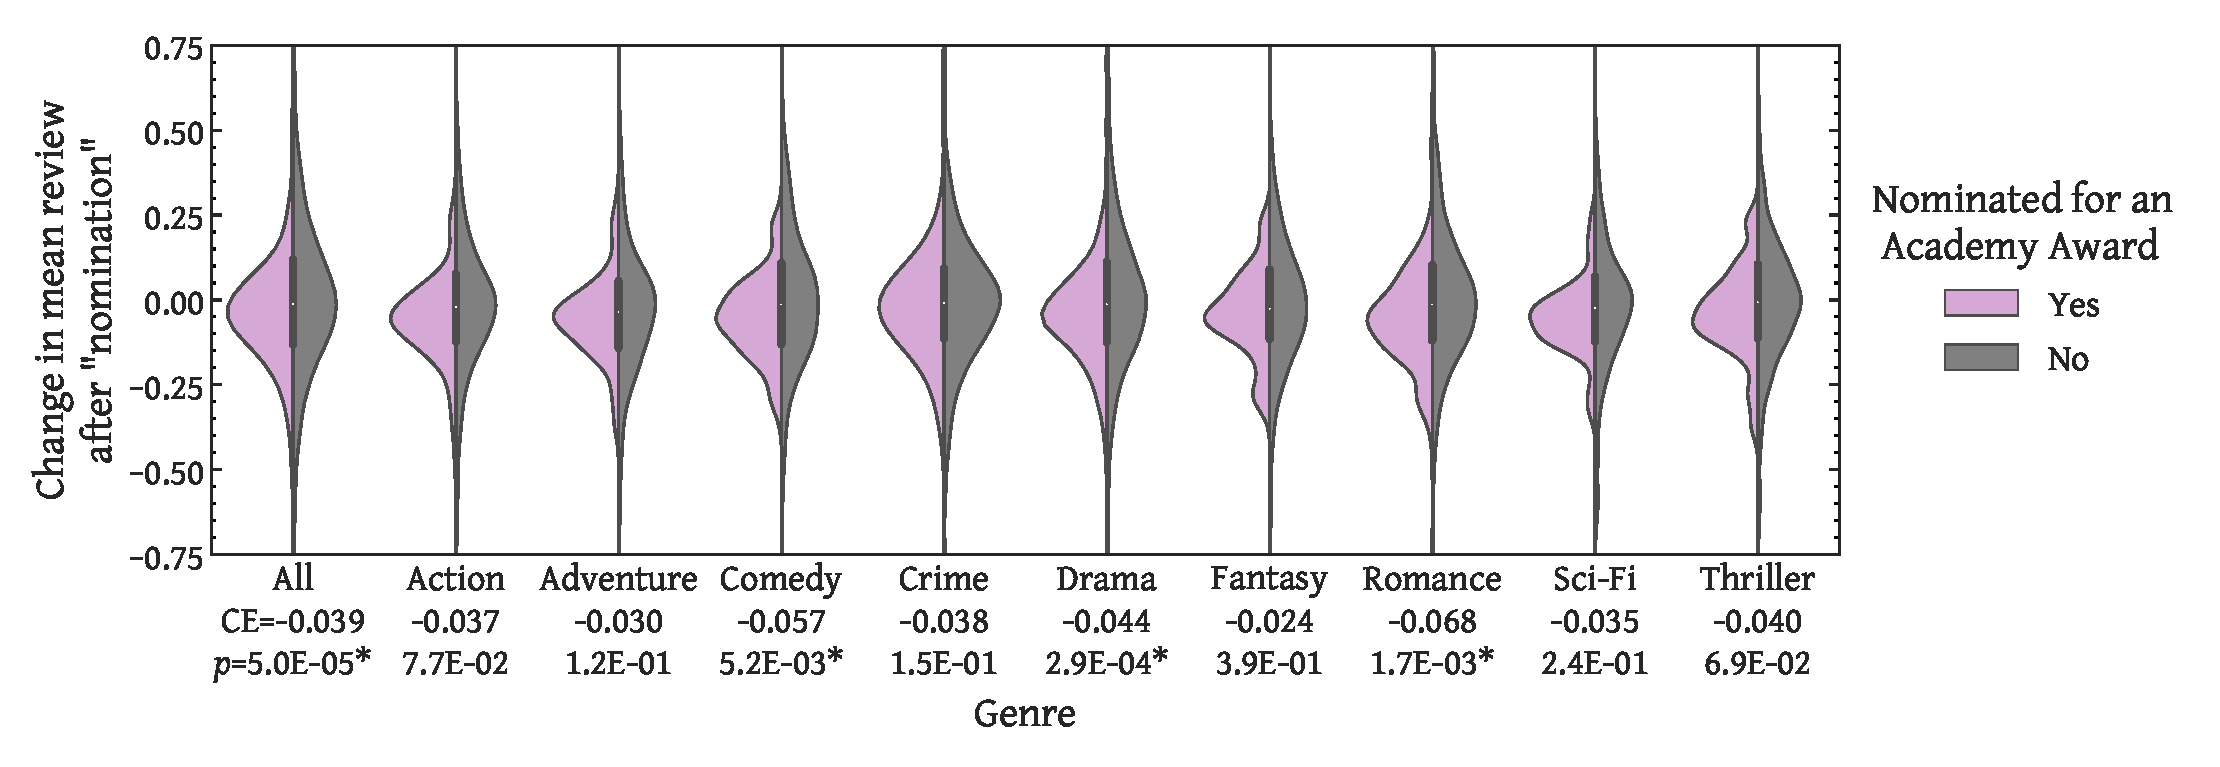
\includegraphics[width=\textwidth]{mc.eps}
    \caption{The causal effect of Oscar nominations on the change in mean rating. The leftmost violin plot corresponds to an aggregate of all genres, whereas the nine violin plots to the right are each for a distinct genre. The distribution of changes in the mean rating of each movie after nomination are displayed for the Oscar-nominated group as well as for those that were not nominated (see Section~\ref{sssec:ce} for how pre- and post-``nomination'' is quantified for movies that were not nominated). In the x-axis labels, CE stands for causal effect as defined in the text.}
    \label{fig:mc}
\end{figure}

\section{Open questions}

The film industry is in a time of upheaval. As consumers shift from traditional media outlets to online, subscription-based services, the classic metrics (i.e., awards and box-office receipts) may no longer be the right way to judge a film. In addition, tech juggernauts such as Amazon, Netflix, and Apple (previously just content distributors) are now developing their own award-winning content. As other, more-traditional content developers begin to establish their own streaming platforms (such as Peacock and Disney+), more fine-grained data about user preferences will become available (although the majority of this data is currently not public). With access to such data, we could extend our analysis, making specific recommendations to production companies about their ongoing projects and identifying areas on which to focus in order to create a competitive online platform.  

Additionally, we were provided movie tag genome data, which provides high-dimensional characterizations of each movie based on user-contributed content. We believe it is worth combining this tag genome data along with user ratings in order to help identify consumer groups based on the movies they have watched and the ratings they have submitted. This is a very challenging problem, as the data is of high dimensionality, the ratings are very sparse, and ratings scores were already partially used when creating the tag genome. Nonetheless, it is interesting to use genome scores as a coordinate system in order to help position future new users' into their best-fitting interest group based on existing information. We made an initial attempt by proposing a two-step imputation-clustering framework, the details of which we include in the Supplementary Information section that follows.

\bibliographystyle{mnras}
\bibliography{bibliography}

\section*{Supplementary Information}

\subsubsection*{Clustering analysis of consumer preferences based on ratings submitted}

This database also contains a \textit{Tag Genome} \citep{TagGenome}, which is a dense matrix that contains ${\sim}$1,100 tag relevance scores for each of ${\sim}$13 thousand movies. Each score ranges from 0 to 1 and describes how relevant a movie is to a particular tag (e.g., \textit{action}, \textit{dark}, \textit{funny}, or \textit{futuristic}). This vector space model was constructed using a \textit{community-supervised learning} approach that employs user-contributed data from MovieLens, including ratings and tags as well as text-based reviews.

We first construct a movie--tag matrix, $\mathbf{MT}$, using the file \texttt{genome-scores.csv} with rows indexed by \textit{movieId}, columns indexed \textit{tagId}, and entries being the genome scores of each movie for each tag. Next, we construct a user--movie matrix, $\mathbf{UM}$, using the file \texttt{rating.csv}, with rows indexed by \textit{userId}, columns indexed by \textit{movieId}, and entries being the rating scores submitted by the users. Both matrices have very high dimensionality and must be reduced before analysis. As a first selection criterion, we only consider movies in the $\mathbf{UM}$ matrix that are also present in the $\mathbf{MT}$ matrix, since there is no tag genome data for the other movies. Next, we only include movies with at least 500 total reviews and users who have submitted at least 500 reviews during the lifetime of their MovieLens account. This step significantly reduces the size of the data, although the resulting $\mathbf{UM}$ matrix is still highly sparse (85\% of the entries are missing). On the other hand, only the \textit{movieId}s of the $\mathbf{MT}$ matrix that are present in the columns of the reduced $\mathbf{UM}$ matrix were as well. The resulting $\mathbf{MT}$ matrix has a shape of $(n_\mathrm{movie}, n_\mathrm{tag}) = (5549, 1128)$ and the $\mathbf{UM}$ matrix has a shape of $(n_\mathrm{user}, n_\mathrm{movie}) = (9239, 5549)$.

The sparsity of the $\mathbf{UM}$ matrix is an issue, since we do not know what rating scores the users would have submitted to the movies that they have not watched (in fact, this is closely related to the problem of building a successful recommendation engine). Here, we choose to proceed with an imputation approach in order to estimate the missing values. We fill the missing rating scores using probabilistic principal component analysis (PPCA), leveraging a software package implemented by one of our team members, Sheridan Green (\href{https://github.com/shergreen/pyppca}{GitHub: shergreen/pyppca}), which follows the method of \citet{ppca}. The PPCA method is a generative data imputation approach based on the notion of a lower-dimensional latent space, the dimension of which we vary between 15 and 50. After this step, $\mathbf{UM}$ is transformed into a dense matrix with no missing values. However, shifting focus to $\mathbf{MT}$, we find that the distribution of genome relevancy scores is heavily skewed towards zero. Therefore, we log-transformed the elements of $\mathbf{MT}$.

\begin{figure}
    \centering
    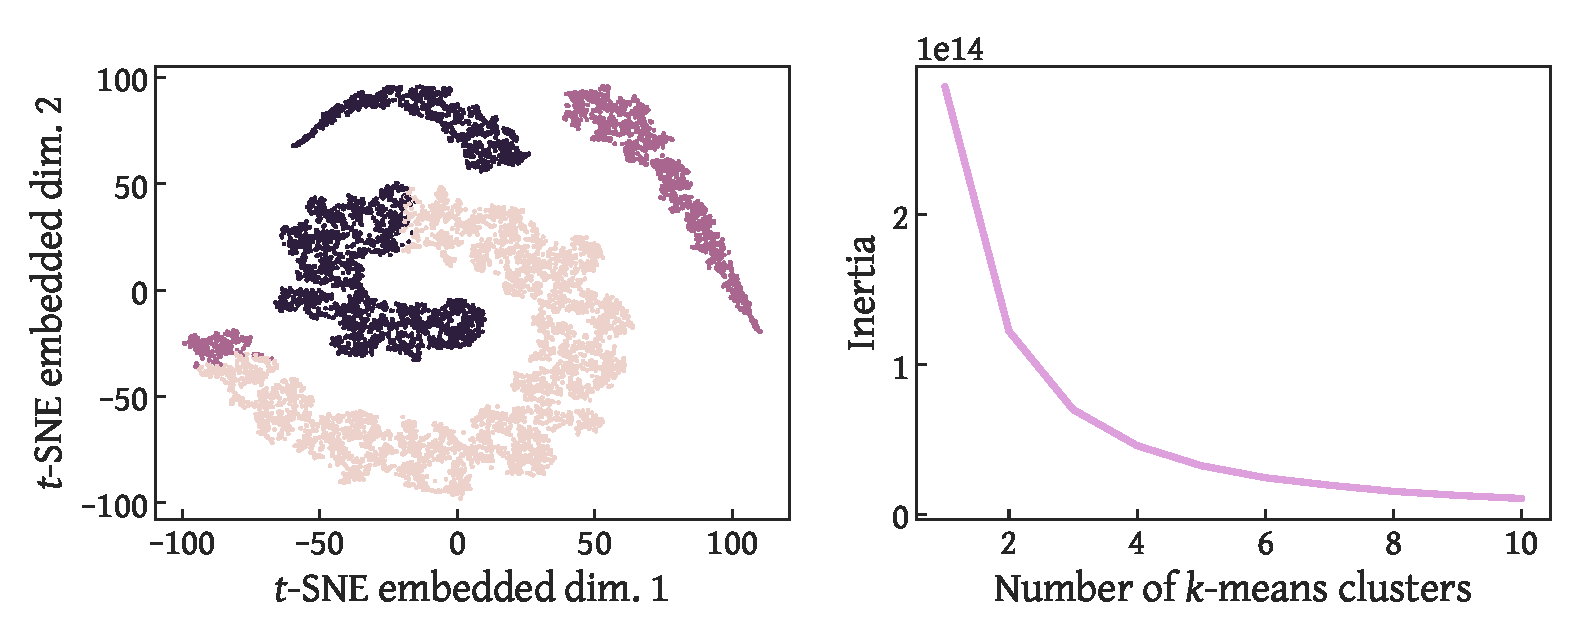
\includegraphics[width=\textwidth]{tsne.eps}\\
    \caption{{\it Left:} The $t$-SNE visualization of the user clusters. {\it Right:} Decay of the $k$-means cost function (inertia, i.e., the sum of squared distances between each point and its cluster centroid) as the number of clusters is increased. The ``elbow method'' suggests an optimal number of clusters is reached at $k=3$.}
    \label{fig:tsne}
\end{figure}

The next step is to represent each user as a vector in the tag coordinate space. The idea is to represent each user by a linear combination of the tag score vectors corresponding to each movie, using the ratings the user submitted (or were imputed) as weights. This leads to a $\mathbf{UT}$ matrix, with rows indexed by \textit{userId}, columns indexed by \textit{tagId}, and entries being the user-rating-weighted sum of movie relevance scores for each tag. According to this definition, the $\mathbf{UT}$ matrix is simply the matrix product of $\mathbf{UM}$ and $\mathbf{MT}$. Note that during our processing steps, after applying the logarithmic transformation, we did not rescale or normalize the scores for each tag in order to avoid reducing the original amount of information contained in $\mathbf{MT}$. Since we use the dense $\mathbf{UM}$ matrix, we do not expect this lack of normalization to yield any problems. The resulting $\mathbf{UT}$ matrix has dimension $(n_\mathrm{user}, n_\mathrm{tag}) = (9239, 1128)$.

Finally, we apply the $k$-means clustering technique with a Euclidean distance metric to the $\mathbf{UT}$ matrix in order to identify potentially existing user groups. Fig.~\ref{fig:tsne} visualizes the clusters using a $t$-SNE plot \citep{tsne} and shows the $k$-means cost function, referred to as inertia (simply the sum of squared distances between each point and its cluster centroid), as the number of clusters is increased. We find that the inertia decays with the number of clusters and that the standard ``elbow method'' suggests the optimal $k = 3$. 

Nonetheless, the separation of the clusters is far from clear and the top tags in each of the three centroids largely overlap, which must be related to the complex geometry of the $\mathbf{MT}$ matrix. Thus, we mention a few promising directions for future exploration: (i) try alternative distance functions for $k$-means in order to better address the issue of high dimensionality (note that the cosine distance is often a better distance metric for comparing the similarity of vectors, but in this case yielded no improvement in our subsequent results); (ii) try alternative imputation techniques to create a dense $\mathbf{UM}$ matrix; (iii) use the sparse rating data but apply a different weighting scheme (see the end of this paragraph); (iv) try selecting users that have given a smaller number of total ratings in order to avoid selecting professional critics and thus analyze only ``normal'' consumers. Still, we believe that clustering consumers based on the data they generate is a promising direction with practical applications for marketing purposes. The success of these clustering methods (as well as content recommendation engines) is highly sensitive to the method used to collect user feedback. When representing users as vector sums of the movies they have watched (in tag space), we must weight the movies based on their preferences. Unfortunately, a five-star rating system is subjective as to whether or not a consumer actually preferred a movie. The cut-off between a rating for a ``good'' movie and a ``bad'' movie will vary from user to user. A binary preference system that consists only of ``like'' and ``dislike'' would likely improve the performance of vector-based consumer modeling, as consumer vectors should be weighted positively towards their preferred films and negatively away from the films they dislike. It would appear that \href{https://about.netflix.com/en/news/goodbye-stars-hello-thumbs}{Netflix came to a similar conclusion}, as they recently switched from a five-star review system to a thumbs up/down system in order to improve their recommendation engine and increase the frequency of user feedback.

\subsubsection*{Identifying trends in subscription-based platforms}

As more of the entertainment industry shifts online, companies will have to adapt their traditional metrics and strategies. For example, Netflix (which now has nearly 200 million subscribers) began as simply a distributor for movies but is now also a competing developer, having spent nearly \$2 billion on original content in 2019.

Unfortunately, most of the data about consumer viewing habits on subscription-based platforms is closely held, making a direct analysis impossible. We therefore use outside data --- scraping a list of Netflix original movies and cross-referencing with the \textit{MovieLens} dataset to understand trends in Netflix content.

We attempted to correlate Netflix's original content production with subscription data pulled from the U.S. Securities and Exchange Commission filings. However, the resulting data (as it is based on quarterly reports) is simply too sparse to extract meaningful correlations. We can expect that consumers will behave differently when choosing a subscription-based platform than they do when simply choosing a film. Therefore, it is interesting to ask the following: why do consumers choose a given platform over another? Given access to more detailed data, we could analyze the extent to which platform content affects actual subscriptions, thus providing valuable insight as companies begin to compete in this new online space.  

\begin{figure}
    \centering
    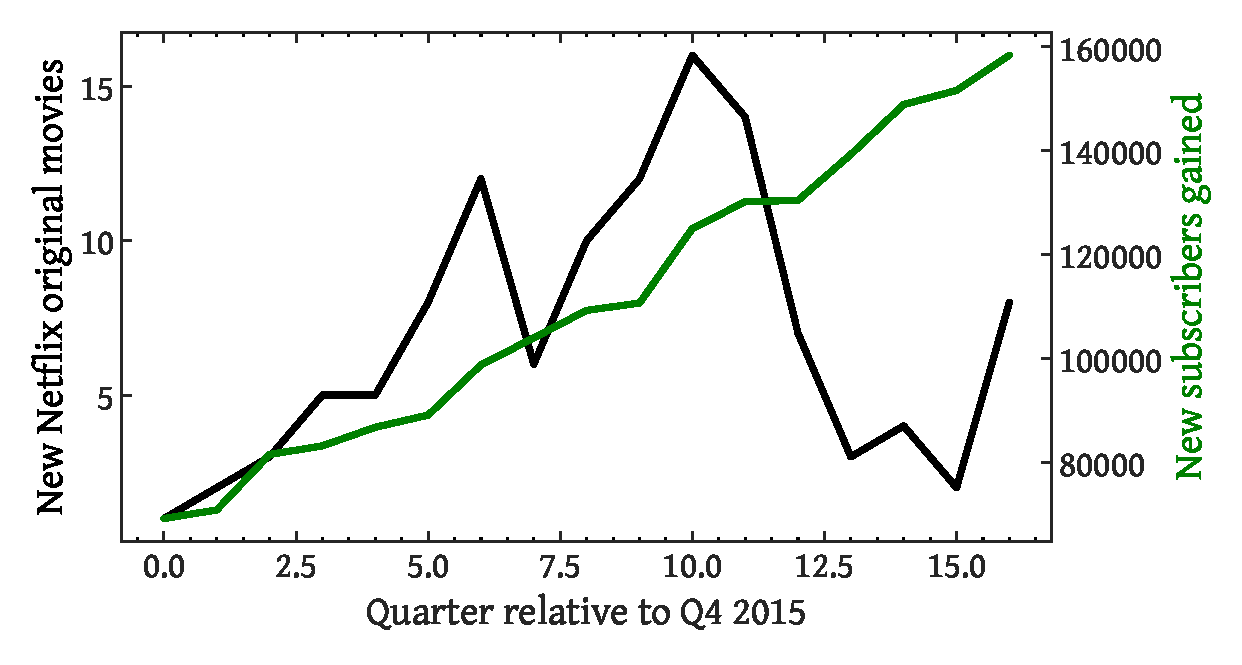
\includegraphics[width=0.55\textwidth]{nsvo.eps}
    \caption{New total quarterly Netflix subscriptions since Q4 2015 and the number of original films released per quarter.}
    \label{fig:nsvo}
\end{figure}

\end{document}